\documentclass{beamer}
%\usetheme{Boadilla}
\usepackage[latin1]{inputenc}
\usepackage{ upgreek }
\usepackage{verbatim} 
\usepackage{amsmath}

\usepackage{array}
\usepackage{amssymb}
\usepackage{graphicx}
\usepackage{url}
\usepackage{verbatim}
\usepackage{multirow} 
\usepackage{relsize}


\usepackage{cite}
\usepackage{url}
\usepackage{color}




\newlength\savedwidth
\newcommand\whline[1]{\noalign{\global\savedwidth\arrayrulewidth
                               \global\arrayrulewidth #1} %
                      \hline
                      \noalign{\global\arrayrulewidth\savedwidth}}
\renewcommand\multirowsetup{\centering}                  


\DeclareMathOperator*{\argmax}{argmax}
\DeclareMathOperator*{\argmin}{argmin}  

\usetheme{Warsaw}
\title{Contextually Guided Semantic Labeling and Search for 3D Point Clouds}




\newcommand{\n}{{n}}             % number of training examples
\newcommand{\x}{{\mathbf x}}     % segmented scene
\newcommand{\xs}[1]{{x_{#1}}}    % segment of scene
\newcommand{\y}{{\mathbf y}}     % labeling of scene
\newcommand{\ys}[1]{{y_{#1}}}    % labeling of segment
\newcommand{\ysc}[2]{{y_{#1}^{#2}}}    % indicator of class label of segment
\newcommand{\zsc}[2]{{z_{#1}^{#2}}}    % indicator of class label pair
\newcommand{\fn}[1]{{\phi_n(#1)}}      % feature function for segment node
\newcommand{\fe}[3]{{\phi_{#1}(#2,#3)}}% feature function for edge
\newcommand{\w}{{\mathbf w}}           % full weight vector
\newcommand{\wn}[1]{{w_n^{#1}}}        % weight vector of segment node
\newcommand{\we}[3]{{w_{#1}^{#2#3}}}   % weight vector of edge
\newcommand{\df}[3]{{f_{#3}(#1,#2)}}   % discriminant function
\newcommand{\loss}[2]{{\Delta(#1,#2)}}   % discriminant function

\newcommand{\wep}[3]{{w_{#1}'^{#2#3}}}   % weight vector of edge
\newcommand{\wnp}[1]{{w_n'^{#1}}}        % weight vector of segment node

\begin{document}
\begin{frame}
\titlepage
\end{frame}

\begin{frame}{Motivation}
	\begin{figure}[t!]
		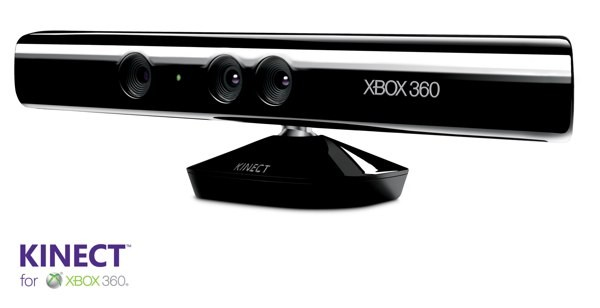
\includegraphics[width=.5\linewidth]{kinect.jpg}
	\end{figure}

	\begin{itemize}
		\item 3D era for robots has arrived 
		\item  cheap, fast 3D machine vision
		\item  both color and depth available
	\end{itemize}

\end{frame}

\begin{frame}{Introduction}
	\begin{itemize}
		\item How does a kinect pointcloud look like? \footnote{http://arstechnica.com/gaming/news/2010/11/bathed-in-light-how-the-kinect-paints-your-room-in-ir-video.ars}

	\end{itemize}
\end{frame}

\begin{frame}{Introduction}
	\begin{itemize}
		\item Desired goal: labeled pointcloud:(show)

	\end{itemize}
\end{frame}

\begin{frame}{Approach}
	\begin{itemize}
		\item stitching:(show animation)
		\item  segmentation:(show)
		\item  graph construction(show using graphviz?)
		\item  feature generation
		\item  inference
	\end{itemize}

\end{frame}

\begin{frame}{Captured Properties}
	\begin{itemize}
		\item Visual Appearance
		\item  Local Shape and Geometry
		\item  Geometrical Context
	\end{itemize}

\end{frame}

\begin{frame}{Visual Appearance}
match the following to table/printer
\begin{figure}[t!]

\includegraphics[width=.3\linewidth]{printer-small.png}
\hskip .2in

\includegraphics[width=.3\linewidth]{table-small.png}
\end{figure}
\end{frame}

\begin{frame}{Visual Appearance}
\begin{figure}[t!]
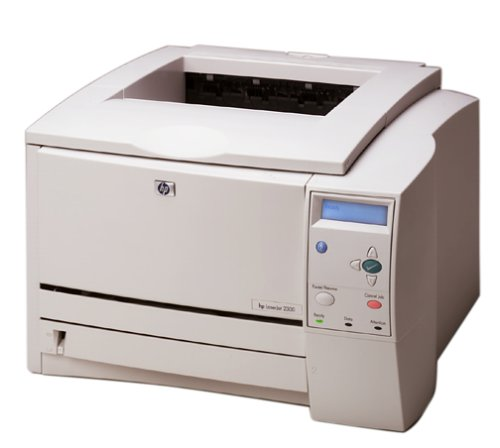
\includegraphics[width=.4\linewidth]{printer.jpg}
\hskip .2in
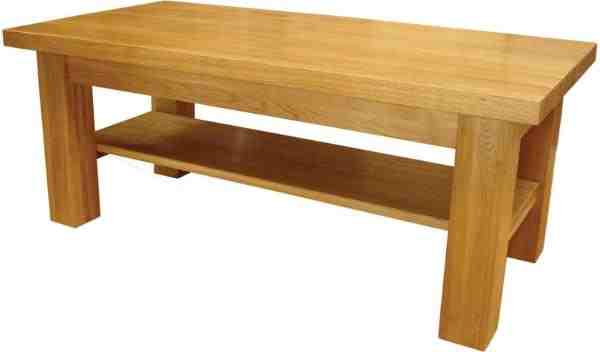
\includegraphics[width=.4\linewidth]{table.jpg}
\end{figure}
\end{frame}



\begin{frame}{Local Shape and Geometry}
\begin{itemize}
\item tableTops are horizontal
\item tableTops are at fixed hights
\item faces of a printer form a convex shape


\end{itemize}

\end{frame}

\begin{frame}{Geometrical Context}
\begin{figure}[t!]
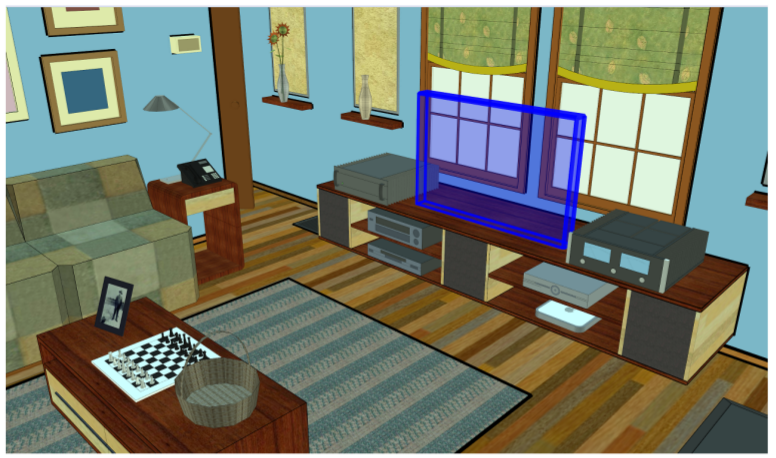
\includegraphics[width=.8\linewidth]{contextHole.png}
\end{figure}
\end{frame}


\begin{frame}{Geometrical Context}
\begin{figure}[t!]
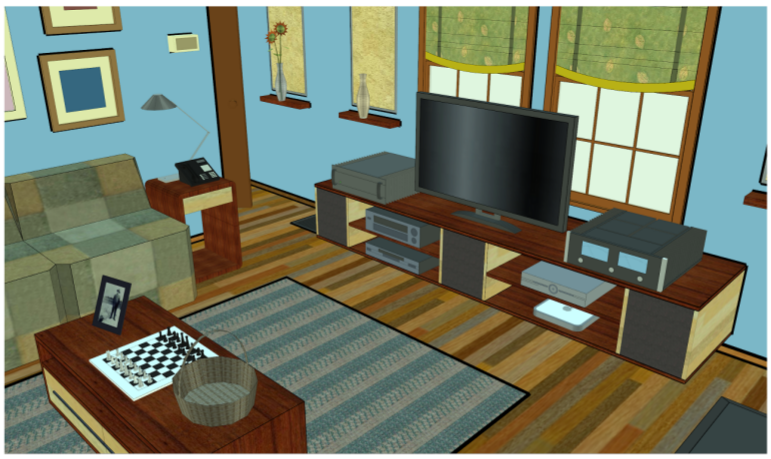
\includegraphics[width=.8\linewidth]{contextHoleFilled.png}
\end{figure}
\end{frame}

\begin{frame}{Model}
\begin{itemize}
 \item The 3D scene is encoded using Markov Random Field with log-linear node and pairwise edge potentials
 \item SHOW CONSTRUCTION GRAPH HERE
 % a small graph with objects in the scene representing nodes and edges?
\end{itemize}
\end{frame}

\begin{frame}{Model}
\begin{itemize}


\item Goal: Given a segmented point cloud $\x=(\xs{1},...,\xs{N})$  predict a labeling $\y=(\ys{1},...,\ys{N})$
\item Number of labels: K
\item where $\ys{i}=(\ysc{i}{1},...,\ysc{i}{K})$,  $ \forall \ysc{i}{k} \in \{0,1\}$ 


\item For a segmented point cloud $\x$, the prediction $\hat{\y}$ is 
\begin{equation} \label{eq:argmax}
\hat{\y} = \argmax_\y \df{\x}{\y}{\w}
\end{equation}

\end{itemize}
\end{frame}


\begin{frame}{Model}
\begin{itemize}

\item Given $(\mathcal{V},\mathcal{E})$, individual segment features $\fn{i}$ and edge features $\fe{t}{i}{j}$

\begin{equation} \label{eq:model}
\begin{split}
\df{\y}{\x}{\w} & = \sum_{i \in \mathcal{V}} \sum_{k=1}^{K} \ysc{i}{k} \left[\wn{k} \cdot \fn{i} \right] \\
 & + \sum_{(i,j)\in \mathcal{E}}   \sum_{l=1}^{K}  \sum_{k=1}^{K} \ysc{i}{l} \ysc{j}{k}  \left[\we{t}{l}{k} \cdot \fe{t}{i}{j}\right] 
 \end{split}
\end{equation}

\end{itemize}
\end{frame}

\begin{frame}{Model}

\begin{itemize}
%There may be multiple types $t$ of edge feature maps $\fe{t}{i}{j}$, and each type has a graph over the $K$ classes with edges $T_t$. If $T_t$ contains an edge between classes $l$ and $k$, then this feature map and a weight vector $\we{t}{l}{k}$ is used to model the dependencies between classes $l$ and $k$. If the edge is not present in $T_t$, then $\fe{t}{i}{j}$ is not used.

\item Multiple types of edge feature maps

\item Visual similarity between segments -- parts of the same object
\item Vertical distance between segment centers -- relates multiple objects
\item IMAGE

\end{itemize}
\end{frame}

\begin{frame}{Model}
\begin{itemize}

\item Each type has a graph over the $K$ classes with edges  $T_t$

\item Associative edges:  ${T_t}=\{(k,k)| \forall k=1..K\}$
\item Non-associative edges: $T_t=\{(l,k)| \forall l,k=1..K\}$
\item Object-associate edges: $T_t=\{(l,k) | \exists object , ~ l,k\in {\rm parts}({\rm object})\}$
\end{itemize}
\hskip 1in
\begin{figure}
		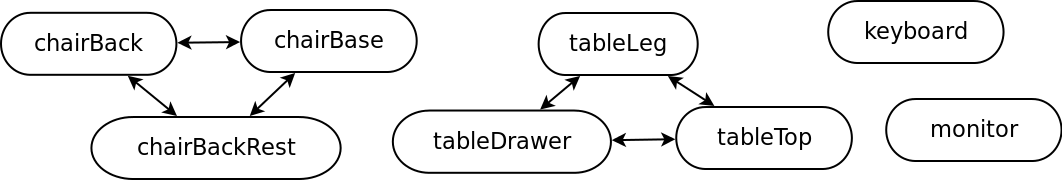
\includegraphics[width=.8\linewidth]{objAssoc.png}
	\end{figure}


\end{frame}

\begin{frame}{Model}
Parsimonious model


%\item Given $(\mathcal{V},\mathcal{E})$, individual segment features $\fn{i}$ and edge features $\fe{t}{i}{j}$

\begin{equation} \label{eq:model}
\begin{split}
\df{\y}{\x}{\w} & = \sum_{i \in \mathcal{V}} \sum_{k=1}^{K} \ysc{i}{k} \left[\wn{k} \cdot \fn{i} \right] \\
 & + \sum_{(i,j)\in \mathcal{E}}   \sum_{T_t \in {\cal T}}  \sum_{(l,k)\in T_t} \ysc{i}{l} \ysc{j}{k}  \left[\we{t}{l}{k} \cdot \fe{t}{i}{j}\right] 
 \end{split}
\end{equation}
\begin{itemize}
\item If $T_t$ contains edge $(l,k)$, then $\fe{t}{i}{j}$ and $\we{t}{l}{k}$  model the dependencies between classes $l$ and $k$.
\item Since $|T_{na}| >> |T_{oa}|$ , the number of parameters to learn is lesser compared to modeling all edges as non-associative.
%\item ``object-associative'' features $\fe{oa}{i}{j}$ - used between classes that are parts of the same object (e.g., ``chair base'', ``chair back'' and ``chair back rest''). 
%\item ``non-associative'' features $\fe{na}{i}{j}$ -  used between any pair of classes.

\end{itemize}
\end{frame}



\begin{frame}{Features}

\begin{itemize}
\item Node Features
\begin{itemize}
\item Visual Appearance
	\begin{itemize}
	\item Histogram of HSV color values
	\item Average HSV color values
	\item HOG features corresponding to the segment
	\end{itemize}
	\item Local Shape and Geometry
	\begin{itemize}
	\item Linear-ness , Planar-ness and Scatter
	\item Vertical component of the normal
	\item Vertical position of centroid
	\item Bounding box dimensions
	\item Distance from scene boundary
	\end{itemize}
\end{itemize}
\end{itemize}

\end{frame}

\begin{frame}{Features}

\begin{itemize}
\item Edge Features
\begin{itemize}
\item Visual Appearance
	\begin{itemize}
	\item Diff in avg. HSV color values
	\end{itemize}
	\item Local Shape and Geometry
	\begin{itemize}
	\item Coplanarity and convexity
	\end{itemize}
	\item Geometric context
	\begin{itemize}
	\item Horizontal distance b/w centroids
	\item Vertical displacement b/w centroids
	\item Angle between normals
	\item Diff in angle with vertical
	\item Distance between closest points
	\item Relative position from camera (in front of/ behind) 
	\end{itemize}
\end{itemize}
\end{itemize}

\end{frame}

\begin{frame}{Inference}
 \begin{eqnarray*}
\hat{\y}\!\!\!&=&\!\!\!\argmax_{\y}\max_{\mathbf z} \sum_{i \in \mathcal{V}} \sum_{k=1}^{K} \ysc{i}{k} \left[\wn{k} \cdot \fn{i} \right] \\
&+&  \!\!\!\sum_{(i,j)\in \mathcal{E}}  \sum_{T_t \in {\cal T}} \sum_{(l,k)\in T_t} \zsc{ij}{lk} \left[\we{t}{l}{k} \cdot \fe{t}{i}{j}\right] 
 \label{eq:relaxobj}\\
\end{eqnarray*}
 \begin{eqnarray*}
  \forall i,j,l,k &:& \:\: \zsc{ij}{lk}\le \ysc{i}{l}, \:\:\:\:
\zsc{ij}{lk}\le \ysc{j}{k},\:\:\:\:
\ysc{i}{l} + \ysc{j}{k} \le \zsc{ij}{lk}+1,\:\:\:\: \\
\forall i &:& \sum_{j=1}^{K} y_i^j = 1\\
\forall i,j,l,k &:& \zsc{ij}{lk},\ysc{i}{l} \in \{ 0,1 \} \label{eq:relaxconst}
\end{eqnarray*}
\end{frame}

\begin{frame}{Learning using $SVM^{struct}$}

\begin{equation} \label{eq:model}
\begin{split}
\df{\y}{\x}{\w} & = \sum_{i \in \mathcal{V}} \sum_{k=1}^{K} \ysc{i}{k} \left[\wn{k} \cdot \fn{i} \right] \\
 & + \sum_{(i,j)\in \mathcal{E}}   \sum_{T_t \in {\cal T}}  \sum_{(l,k)\in T_t} \ysc{i}{l} \ysc{j}{k}  \left[\we{t}{l}{k} \cdot \fe{t}{i}{j}\right] \\
& = \w^T \Psi(\x,\y)
 \end{split}
\end{equation}
where, $\Psi(\x,\y)=XY$

\end{frame}

\begin{frame}{Learning using $SVM^{struct}$}
learn weights w such that $\w^T \Psi(\x,\y)$  is max for correct y
\begin{figure}[t!]
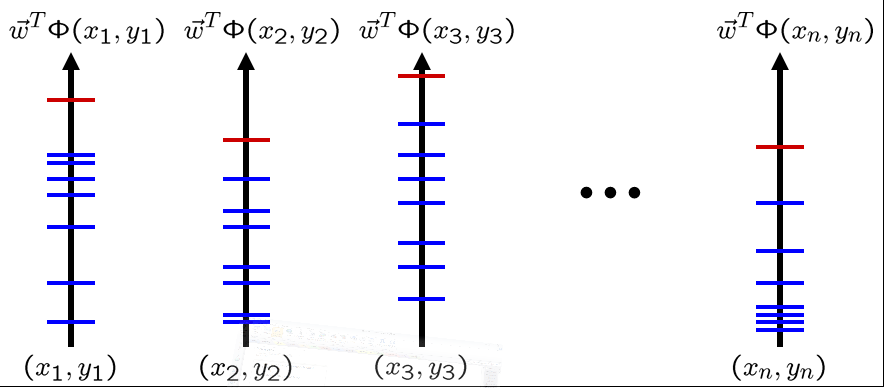
\includegraphics[width=.9\linewidth]{struct.png}
\end{figure}
\end{frame}


\begin{frame}{Learning using $SVM^{struct}$}
\begin{eqnarray} \label{eq:trainqp}
\min_{w,\xi}    \frac{1}{2} \w^T\w + C\xi\\
s.t.   \forall \bar{\y}_1,...,\bar{\y}_\n \in \{0,0.5,1\}^{N \cdot K} :\\
 \frac{1}{n} \w^T \sum_{i=1}^{n} [\Psi( \x_i, \y_i) \nonumber - \Psi(\x_i,\bar{\y}_i)] \ge \Delta(\y_i,\bar{\y}_i) -\xi \nonumber
\end{eqnarray}

\begin{itemize}
\item convex quadratic program
\item $3^{N.K}$ constraints!
\end{itemize}
\end{frame}

\begin{frame}{Learning algorithm}
Thorsten's slides
\end{frame}


\begin{frame}{Inference for Learning}
 \begin{eqnarray*}
\hat{\y}\!\!\!&=&\!\!\!\argmax_{\y}\max_{\mathbf z} \sum_{i \in \mathcal{V}} \sum_{k=1}^{K} \ysc{i}{k} \left[\wn{k} \cdot \fn{i} \right] \\
&+&  \!\!\!\sum_{(i,j)\in \mathcal{E}}  \sum_{T_t \in {\cal T}} \sum_{(l,k)\in T_t} \zsc{ij}{lk} \left[\we{t}{l}{k} \cdot \fe{t}{i}{j}\right] \\
&+& \color<0-1>{red}{\loss{\y_i}{\y}} \label{eq:relaxobj}\\
\end{eqnarray*} 

\begin{eqnarray*}
\forall i,j,l,k &:& \:\: \zsc{ij}{lk}\le \ysc{i}{l}, \:\:\:\:
\zsc{ij}{lk}\le \ysc{j}{k},\:\:\:\:
\ysc{i}{l} + \ysc{j}{k} \le \zsc{ij}{lk}+1,\:\:\:\: \\
\invisible<2->
{\forall i,j,l,k &:& \zsc{ij}{lk},\ysc{i}{l} \in \{ 0,1 \} \label{eq:relaxconst}\\}
\uncover<2->
{\forall i,j,l,k &:& \zsc{ij}{lk},\ysc{i}{l} \in [ 0,1 ] \label{eq:relaxconst}\\}
\invisible<3->
{\forall i &:& \sum_{j=1}^{K} y_i^j = 1\\}
\end{eqnarray*} 

\end{frame}

\begin{frame}{Inference for Learning}
 \begin{eqnarray*}
\hat{\y}\!\!\!&=&\!\!\!\argmax_{\y}\max_{\mathbf z} \sum_{i \in \mathcal{V}} \sum_{k=1}^{K} \ysc{i}{k} \left[\wn{k} \cdot \fn{i} \right] \\
&+&  \!\!\!\sum_{(i,j)\in \mathcal{E}}  \sum_{T_t \in {\cal T}} \sum_{(l,k)\in T_t} \zsc{ij}{lk} \left[\we{t}{l}{k} \cdot \fe{t}{i}{j}\right] \\
&+& \loss{\y_i}{\y} \label{eq:relaxobj}\\
\forall i,j,l,k &:& \:\: \zsc{ij}{lk}\le \ysc{i}{l}, \:\:\:\:
\zsc{ij}{lk}\le \ysc{j}{k},\:\:\:\:
\ysc{i}{l} + \ysc{j}{k} \le \zsc{ij}{lk}+1,\:\:\:\: \\
\forall i &:& \sum_{j=1}^{K} y_i^j = 1\\
\forall i,j,l,k &:& \zsc{ij}{lk},\ysc{i}{l} \in [ 0,1 ] \label{eq:relaxconst}
\end{eqnarray*} 

\begin{itemize}
 \item $y_i^k\in{0,0.5,1}$
 \item can be also solved by QBPO(which uses graph-cut)
\end{itemize}

\end{frame}


\begin{frame}{Data}
% types and number of scene 
% examples of labeled pointclouds
\begin{itemize}
   \item Two types of indoor environments : 
   \begin{itemize}
   \item Office 
   	\begin{itemize}
	\item 24 stitched scenes
	\item 1108 labeled segments
	\item wall, floor, tableTop, tableDrawer, tableLeg, chairBackRest, chairBase, chairBack, monitor, printerFront, printerSide keyboard, cpuTop, cpuFront, cpuSide, book, paper
	\end{itemize}
   \item Home
   	\begin{itemize}
   	\item  28 stitched scenes
	\item 1387 labeled segments
	\item wall, floor, tableTop, tableDrawer, tableLeg, chairBackRest, chairBase, sofaBase, sofaArm, sofaBackRest, bed, bedSide, quilt, pillow, shelfRack, laptop, book 
	\end{itemize} 
\end{itemize}
\end{itemize}
\end{frame}


\begin{frame}{Results }
% put table
% put confusion matrices 
% discuss the points mentioned in the paper  


\begin{table}

\caption{{\bf Learning experiment statistics.} The table shows average micro precision/recall, and average macro precision and recall for home and office scenes. }
 %\label{tbl:overall_result}
 
{\tiny
\newcolumntype{P}[2]{>{\footnotesize#1\hspace{0pt}\arraybackslash}p{#2}}
\setlength{\tabcolsep}{2pt}
\centering
\resizebox{\hsize}{!}
 {
\begin{tabular}
{p{0.24\linewidth}p{0.16\linewidth}|P{\centering}{14mm}P{\centering}{12mm}P{\centering}{12mm}|P{\centering}{14mm}P{\centering}{12mm}P{\centering}{12mm} }\\
%{p{0.15\linewidth}p{0.18\linewidth}|p{10mm}p{12mm}p{12mm}|p{12mm}p{12mm}p{12mm}|p{12mm}p{12mm}p{12mm}|p{12mm}p{10mm}p{12mm}p{12mm}p{12mm}p{12mm}}
%\multicolumn{18}{c}{Listed environment-wise, averaged over the objects.} \\
\whline{1.1pt} 

& & \multicolumn{3}{c|}{Office Scenes} & \multicolumn{3}{c}{Home Scenes}  \\
\cline{3-8}
& & \multicolumn{1}{c}{micro} & \multicolumn{2}{c|}{macro} & \multicolumn{1}{c}{micro} &  \multicolumn{2}{c}{macro}   \\
\whline{0.4pt} 

     features &  algorithm & \multicolumn{1}{c}{$P/R$} & \multicolumn{1}{c}{Precision}  & \multicolumn{1}{c|}{Recall} &  \multicolumn{1}{c}{$P/R$} & \multicolumn{1}{c}{Precision} &  \multicolumn{1}{c}{Recall}  \\ 
\whline{0.8pt} 

None &  chance &  26.23 & 5.88 & 5.88 & 29.38 & 5.88 & 5.88\\
\whline{0.6pt} 

Image Only &           svm\_node\_only                        & 46.67  & 35.73 & 31.67 &   38.00 & 15.03 & 14.50\\%  &  &  &     \\
Shape Only &              svm\_node\_only                        & 75.36  & 64.56 & 60.88 &    56.25 & 35.90 & 36.52 \\
% &  &  &    \\
Image+Shape &         svm\_node\_only                         & 77.97  & 69.44 & 66.23 &   56.50 & 37.18 & 34.73 \\
% &  &  &   \\
\whline{0.6pt}

Image+Shape \& context &  single\_frames                 & 84.32 & 77.84 & 68.12 & 69.13 & 47.84 & 43.62 \\
%Image+Shape \& context &  single\_frames 500                 & 70.37 & 62.88 & 47.27 &  &  &  \\
%Image+Shape \& context &  single\_frames 500,sum$\le$1                 & 77.57/63.35 & 63.58 & 36.51 &  &  &  \\
%Image+Shape \& context &  single\_frames 500,learn,sum1                 & 78.36 & 68.86 & 66.69 &  &  &  \\
%Image+Shape \& context &  single\_frames, sum$\le$1                 & 89.27/55.17 & 74.29 & 35.24 & 82.09/52.35 & 52.03 &  26.22 \\

%  &  &  &    \\
\whline{0.6pt} 

Image+Shape \& context &  svm\_mrf\_assoc   					& 75.94  & 63.89 & 61.79 &    62.50 & 44.65 & 38.34\\
%  & &  &   \\
Image+Shape \& context &  svm\_mrf\_nonassoc   					& 81.45  &76.79  &70.07   & 72.38  & 57.82  & 53.62 \\
% &   &  &    \\
Image+Shape \& context &  svm\_mrf\_parsimon	     			& 84.06  & 80.52  & 72.64   & 73.38  & 56.81  &54.80 \\
%  &  &   \\

\whline{1.1pt} 

\end{tabular}
}
}

\end{table}
{\small
\begin{itemize}
\item Do image and point-cloud features capture complimentary information? 
\item How	important	is context?
\item How does a full 3D model compare to a 2.5D model?
\end{itemize}
}
\end{frame}

\begin{frame}{Results}
Confusion Matrix for Office dataset
  \begin{figure}
		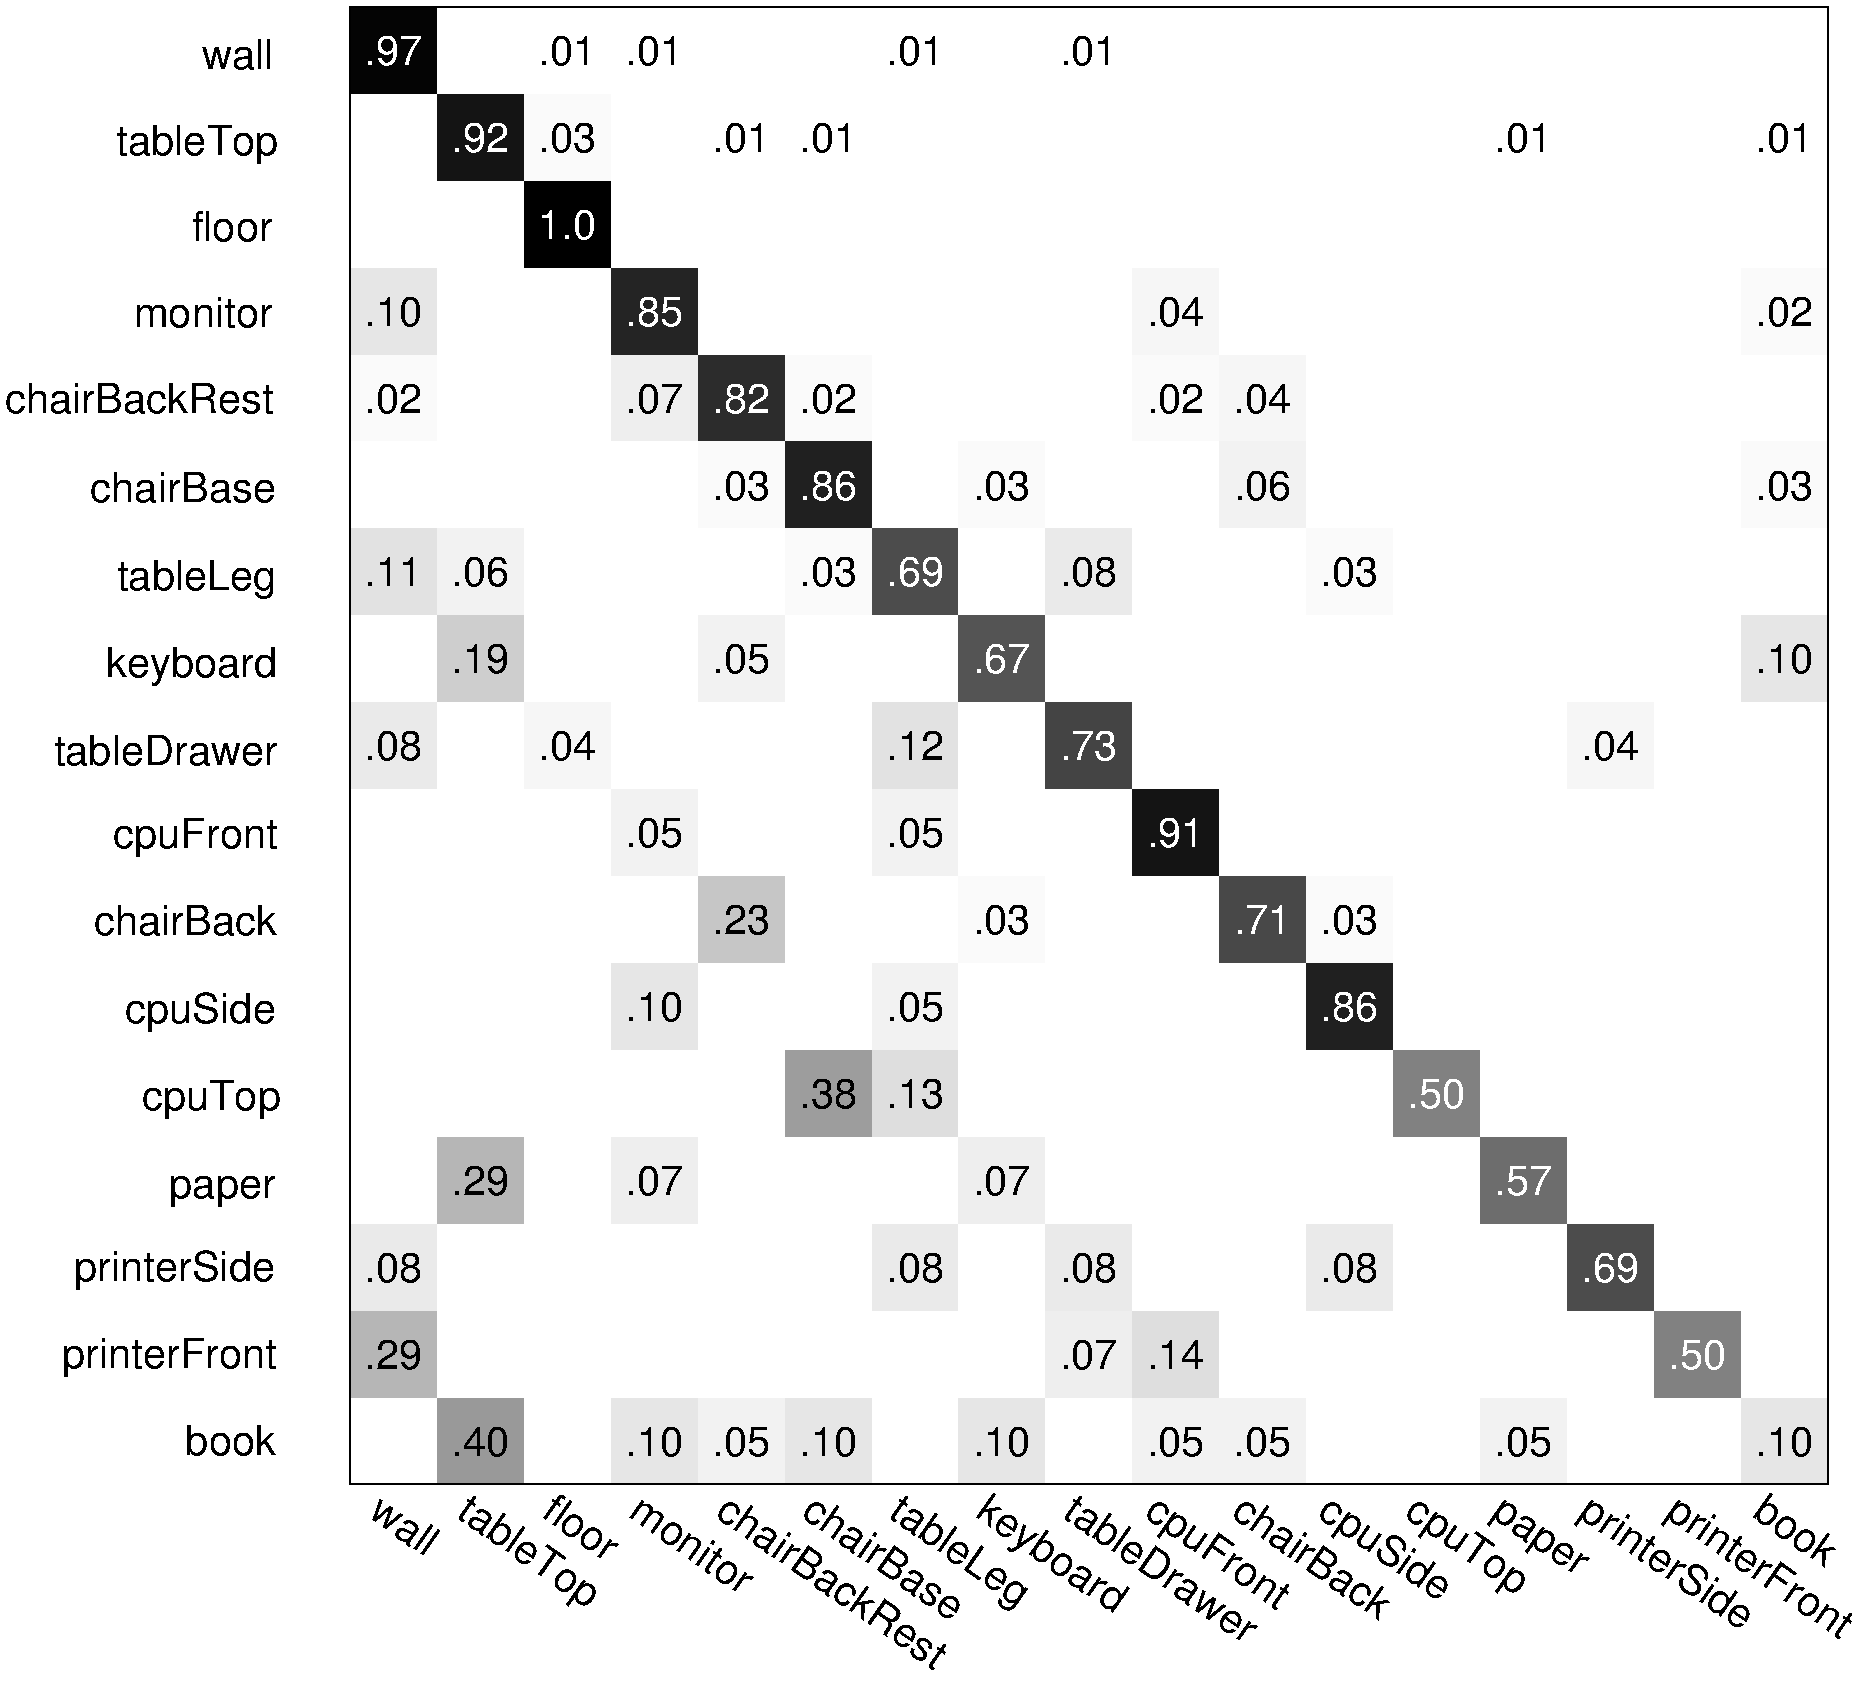
\includegraphics[scale=0.2]{objassoc_office_radius0_6.pdf} 
	\end{figure}

\end{frame}

\begin{frame}{Results}
Confusion Matrix for Home dataset
 \begin{figure}   
 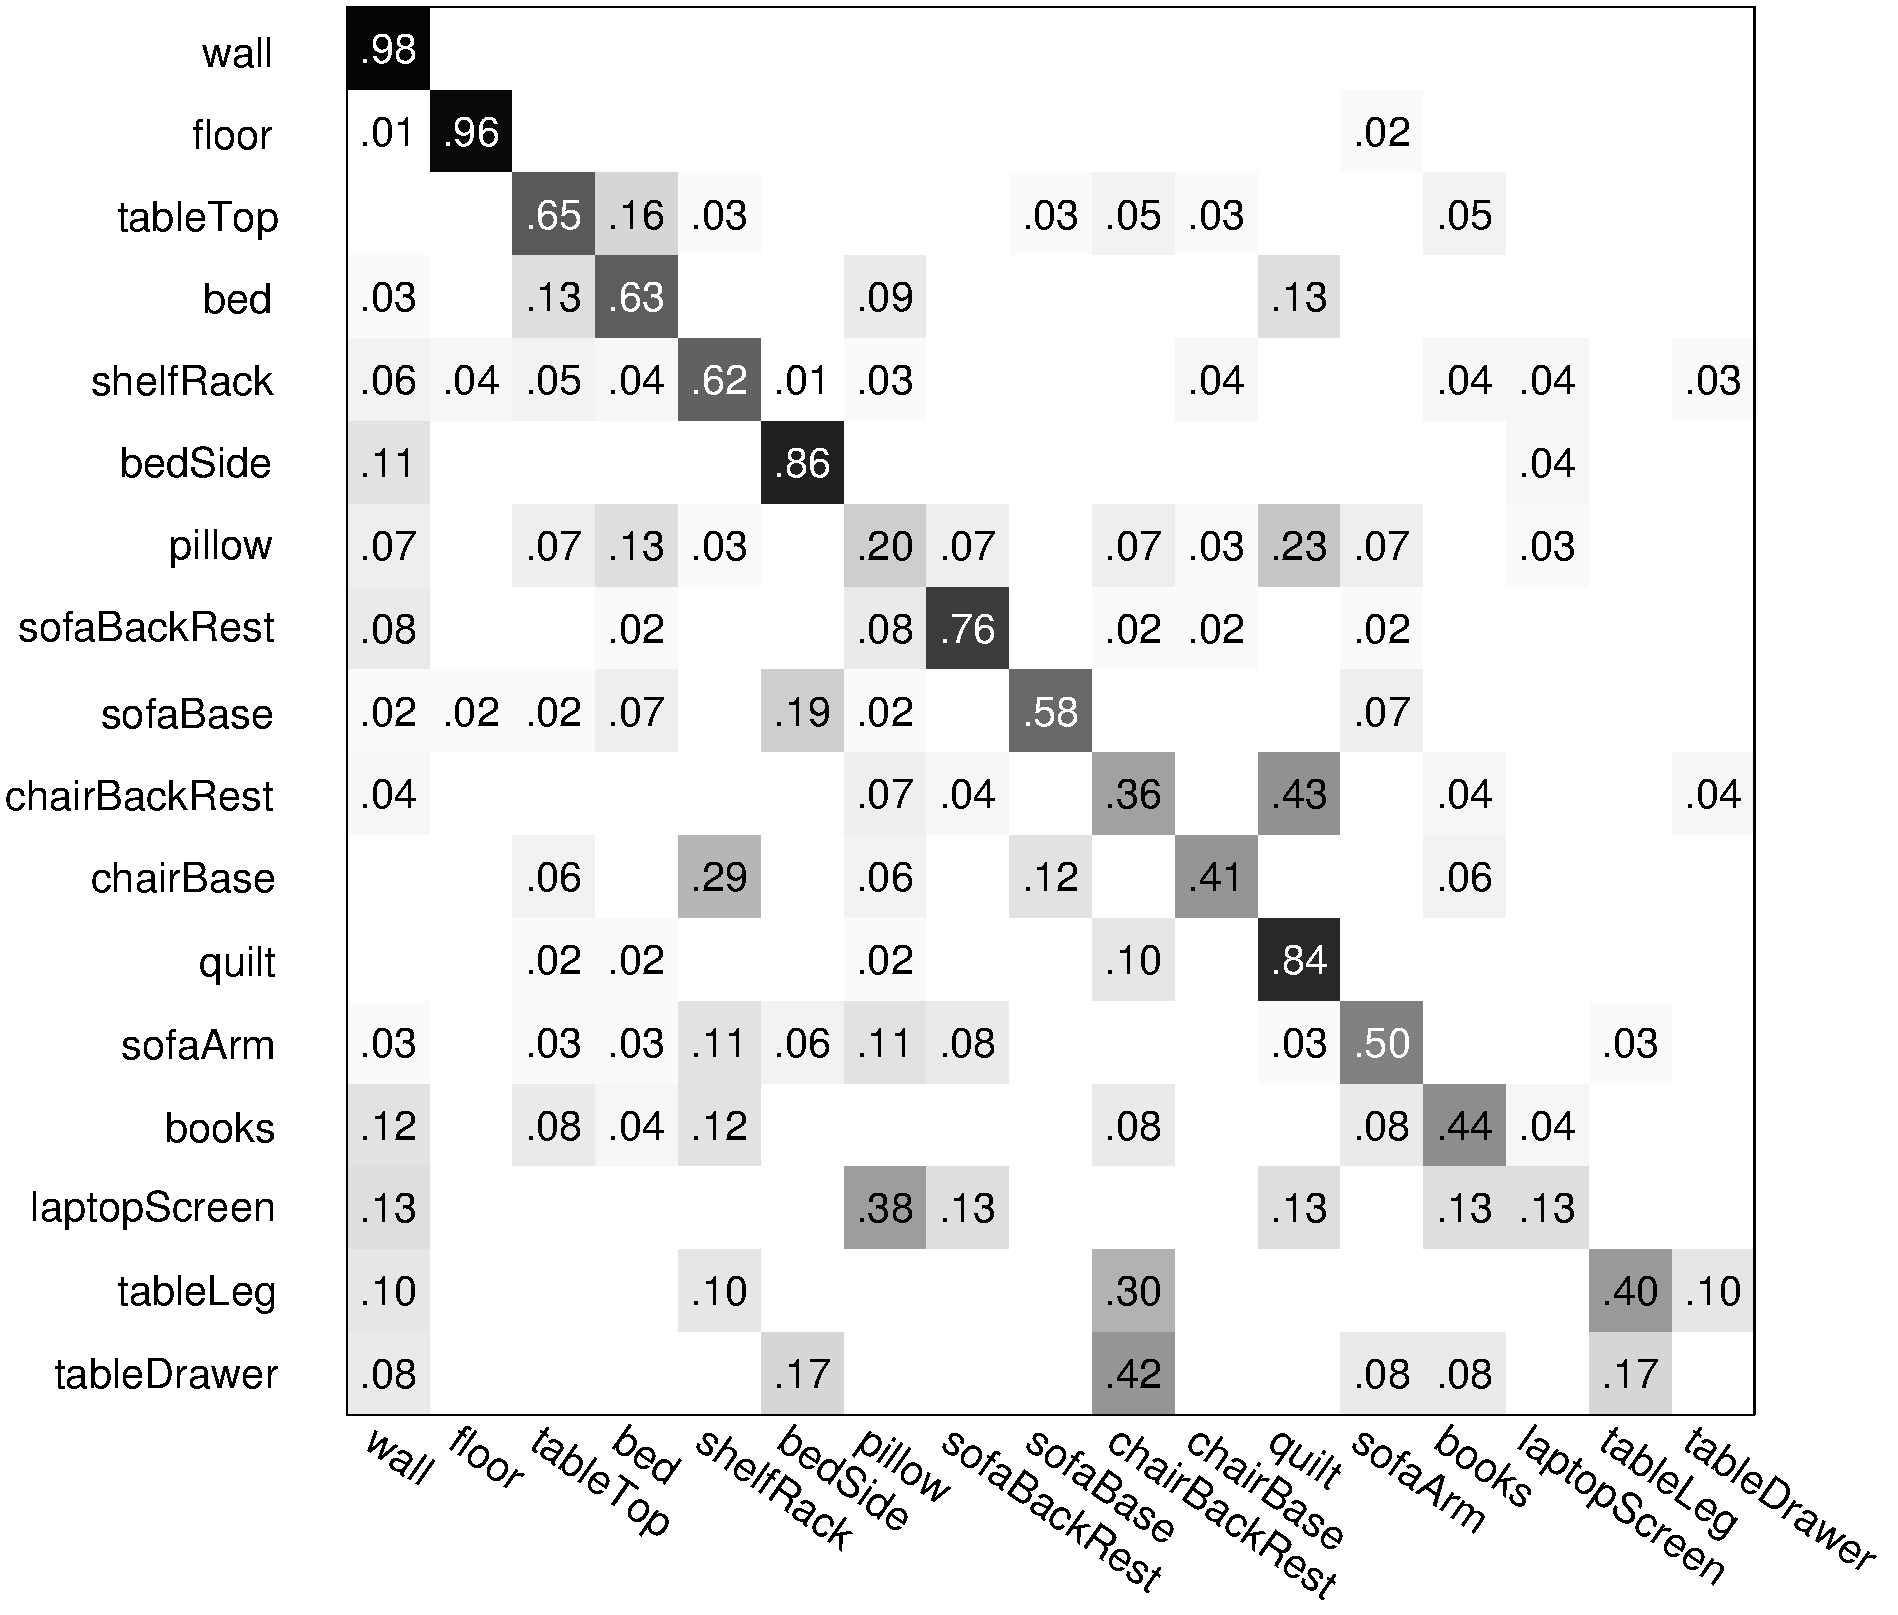
\includegraphics[scale=0.2]{objassoc_home_radius0_6.pdf} 
 \end{figure}
\end{frame}

\begin{frame}{Results}
How large should the Context Range be?
  \begin{figure}
	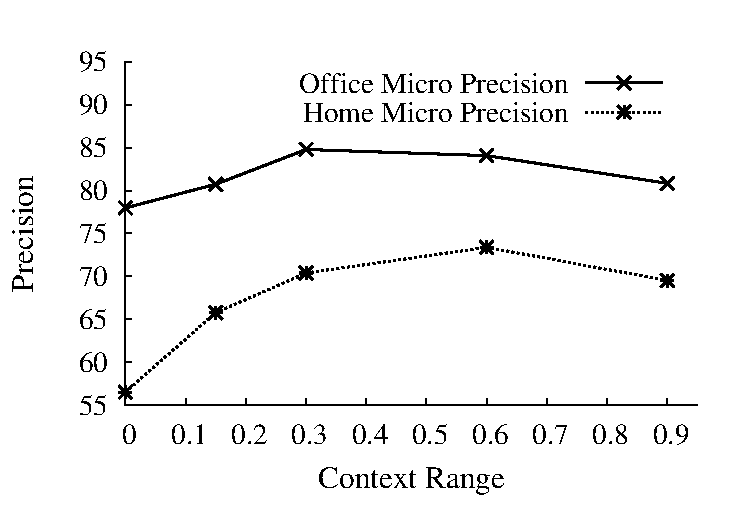
\includegraphics[scale=0.5]{radiusEffectPlot.pdf} 
  \end{figure}
\end{frame}

\begin{frame}{Putting it on the robot}

\begin{itemize}
\item the world has more than 17 classes
\item what if an object is not found
\end{itemize}

\end{frame}

\begin{frame}{The world has more than 17 classes}
 \begin{eqnarray*}
\hat{\y}\!\!\!&=&\!\!\!\argmax_{\y}\max_{\mathbf z} \sum_{i \in \mathcal{V}} \sum_{k=1}^{K} \ysc{i}{k} \left[\wn{k} \cdot \fn{i} \right] \\
&+&  \!\!\!\sum_{(i,j)\in \mathcal{E}}  \sum_{T_t \in {\cal T}} \sum_{(l,k)\in T_t} \zsc{ij}{lk} \left[\we{t}{l}{k} \cdot \fe{t}{i}{j}\right] \\
&+& \loss{\y_i}{\y} \label{eq:relaxobj}\\
\forall i,j,l,k &:& \:\: \zsc{ij}{lk}\le \ysc{i}{l}, \:\:\:\:
\zsc{ij}{lk}\le \ysc{j}{k},\:\:\:\:
\ysc{i}{l} + \ysc{j}{k} \le \zsc{ij}{lk}+1,\:\:\:\: \\
\forall i,j,l,k &:& \zsc{ij}{lk},\ysc{i}{l} \in [ 0,1 ] \label{eq:relaxconst}\\
\forall i &:& \sum_{j=1}^{K} y_i^j = 1
\end{eqnarray*} 

\end{frame}



\begin{frame}{The world has more than 17 classes}
 \begin{eqnarray*}
\hat{\y}\!\!\!&=&\!\!\!\argmax_{\y}\max_{\mathbf z} \sum_{i \in \mathcal{V}} \sum_{k=1}^{K} \ysc{i}{k} \left[\wn{k} \cdot \fn{i} \right] \\
&+&  \!\!\!\sum_{(i,j)\in \mathcal{E}}  \sum_{T_t \in {\cal T}} \sum_{(l,k)\in T_t} \zsc{ij}{lk} \left[\we{t}{l}{k} \cdot \fe{t}{i}{j}\right] \\
&+& \loss{\y_i}{\y} \label{eq:relaxobj}\\
\forall i,j,l,k &:& \:\: \zsc{ij}{lk}\le \ysc{i}{l}, \:\:\:\:
\zsc{ij}{lk}\le \ysc{j}{k},\:\:\:\:
\ysc{i}{l} + \ysc{j}{k} \le \zsc{ij}{lk}+1,\:\:\:\: \\
\forall i,j,l,k &:& \zsc{ij}{lk},\ysc{i}{l} \in [ 0,1 ] \label{eq:relaxconst} \\
\forall i &:& \sum_{j=1}^{K} y_i^j \le 1
\end{eqnarray*} 
\end{frame}


\begin{frame}{The world has more than 17 classes}
\begin{itemize}
\item Results on the two datasets using the above inference method:
\end{itemize}

\begin{center}
\begin{tabular}{c | c | c | c | c}
Data & Micro-  & Micro-  & Macro-  & Macro-\\
 &  precision &  recall &  precision &  recall\\
\hline
Office & 89.27 & 55.17 & 74.29 & 35.24 \\
Home & 82.09 & 52.35 & 52.03 & 26.22 \\
\hline
\end{tabular}
\end{center}
\end{frame}


\begin{frame}{What if an object in not found?}
\begin{itemize}
\item Find the most contextually likely location by imagining an segment at every discretized 3D location.
\end{itemize}
 \begin{figure}   
 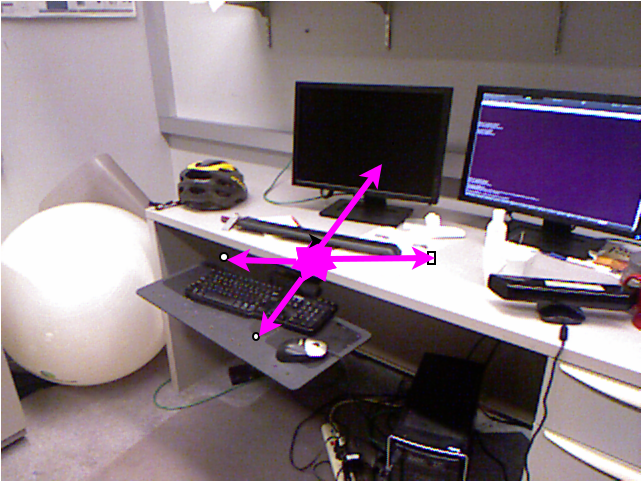
\includegraphics[scale=0.3]{heatImage.png} 
 \end{figure}

\end{frame}


\begin{frame}{Robotic Experiments}

% setup
%demo
% table of results
\begin{itemize}
\item Goal : Robot is asked to find a set of object classes in an office scene.
\item Start at a predetermined location. 
\item Scan room by turning a fixed angle.
\item Classify and save the labeled point clouds. 
\item Find contextually likely locations for object classes not found.
\item Move to the predicted locations and obtain new point clouds.
\item Update predicted locations when new objects are found.
\item Stop when all object classes are found.

\end{itemize}

\end{frame}

\begin{frame}{Robotic Experiments: Results}

\begin{itemize}

\item Results for finding 12 object classes in 10 office scenes

\end{itemize}

\begin {center}
{\footnotesize 
\begin{tabular}{c | c | c | c}
class & precision & recall & \# instances\\
\hline
Wall  & 100 & 100 & 10\\
Table Top  & 100  &100 & 10 \\
Table Leg & 71.43 & 50 & 10 \\
Table Drawer & 100 & 71.43 & 7\\
Chair Backrest & 100 & 100 & 10 \\
Chair Base & 100  & 100 & 10 \\
Chair Back & 100 & 87.5 & 8 \\
Monitor & 100 & 100 & 9 \\
Keyboard & 100 & 77.7 & 9\\
CPU & 50 & 11.1 & 8 \\ 
Printer & 100 & 100 & 1\\
Paper & 100 & 22.2 & 10\\
\hline
Overall Micro & 96.15 & 75 \\
Overall Macro & 93.45 & 76.66 \\

\end{tabular}
}
\end{center}

\end{frame}

\begin{frame}{Current Work: Using grammars for scene understanding}


\end{frame}

\begin{frame}{Current Work: Object Affordance Detection via Human Demonstration}
\begin{itemize}
\item Affordances :  properties of the environment that afford a certain action to be performed by a human or an animal
\end{itemize}
\begin{figure}[t!]
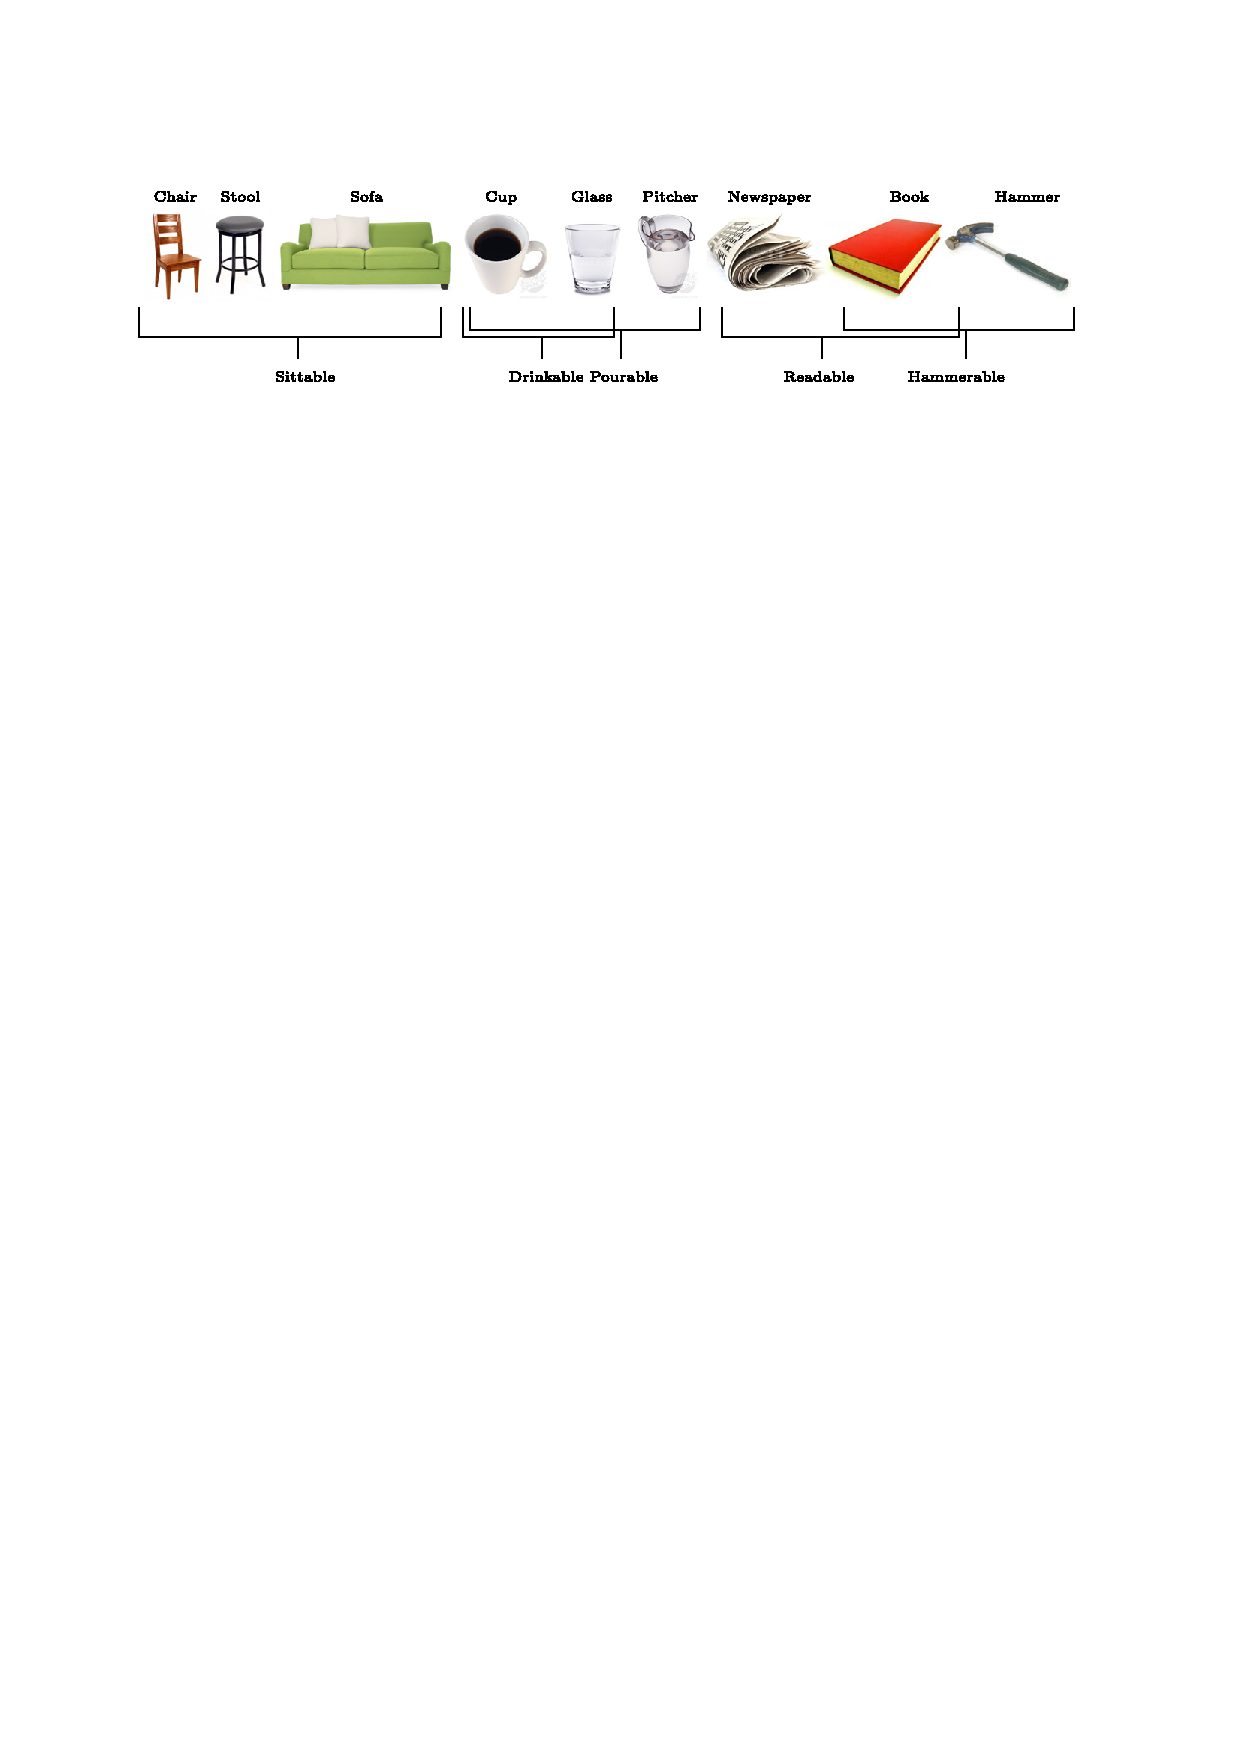
\includegraphics[width=.95\linewidth]{affordances.pdf}
\end{figure}
\end{frame}

\begin{frame}{Object Affordance Detection via Human Demonstration}
\begin{itemize}
\item Human-Object interactions: Affordance depends on human-poses / sub-actions
\end{itemize}
\begin{figure}[t!]
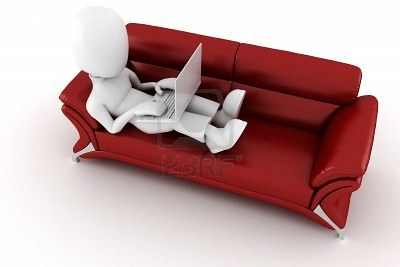
\includegraphics[width=.25\linewidth]{couch_sit.jpg}
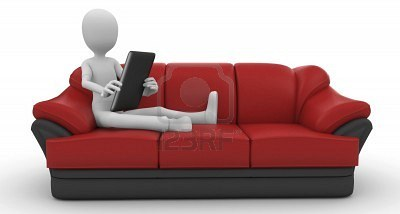
\includegraphics[width=.25\linewidth]{couch_read.jpg}
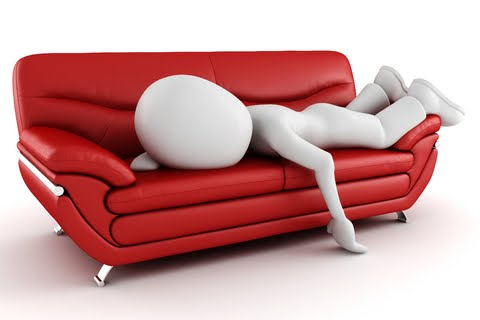
\includegraphics[width=.25\linewidth]{couch_sleep.jpg}
\end{figure}
\begin{itemize}
\item Object-Object interactions: Affordance of objects are related
\end{itemize}
\begin{figure}[h]
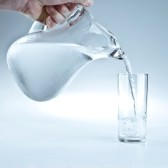
\includegraphics[width=.25\linewidth]{pitcher-pouring.jpg}
\end{figure}
\end{frame}

\begin{frame}{Object Affordance Detection via Human Demonstration}
\begin{itemize}
\item 
\end{itemize}

\end{frame}

\end{document} 
